\documentclass[12pt,a4paper]{report}

%adjust your page margins here
\usepackage[top=0.70in, bottom=0.70in, left=0.8in,right=0.80in]{geometry} % setting the page alignment with this package
\usepackage[pdftex]{graphicx} %for embedding images
\usepackage[dvips, bookmarks,  colorlinks=false]{hyperref} %for creating links in the pdf version and other additional pdf attributes, no effect on the printed document
\hypersetup{%
    pdfborder = {0 0 0}
}
\usepackage[final]{pdfpages} %for embedding another pdf, remove if not required
\usepackage{float} %used for figure placement with H as a parameter
\usepackage{hyperref}
\usepackage{pslatex} % for times new roman, old package, but works
\usepackage{array} % for making text bold in table
\usepackage{setspace}
\usepackage{float}
\usepackage{enumerate}
\usepackage{longtable}
\usepackage{verbatim}

\usepackage[font=small,labelfont=bf]{caption}
\def\figurename{\textbf{Figure }}

\usepackage{listings}
\usepackage{color}

\definecolor{dkgreen}{rgb}{0,0.6,0}
\definecolor{gray}{rgb}{0.5,0.5,0.5}
\definecolor{mauve}{rgb}{0.58,0,0.82}
 
\lstset{ %
  language=Java,                % the language of the code
  basicstyle=\footnotesize,           % the size of the fonts that are used for the code
  numbers=left,                   % where to put the line-numbers
  numberstyle=\tiny\color{gray},  % the style that is used for the line-numbers
  stepnumber=1,                   % each line is numbered
  numbersep=5pt,                  % how far the line-numbers are from the code
  backgroundcolor=\color{white},      % choose the background color. You must add \usepackage{color}
  showspaces=false,               % show spaces adding particular underscores
  showstringspaces=false,         % underline spaces within strings
  showtabs=false,                 % show tabs within strings adding particular underscores
  frame=single,                   % adds a frame around the code
  rulecolor=\color{black},        % if not set, the frame-color may be changed on line-breaks within not-black text (e.g. commens (green here))
  tabsize=2,                      % sets default tabsize to 2 spaces
  captionpos=b,                   % sets the caption-position to bottom
  breaklines=true,                % sets automatic line breaking
  breakatwhitespace=false,        % sets if automatic breaks should only happen at whitespace
  title=\lstname,                   % show the filename of files included with \lstinputlisting;
                                  % also try caption instead of title
  keywordstyle=\color{blue},          % keyword style
  commentstyle=\color{dkgreen},       % comment style
  stringstyle=\color{mauve},         % string literal style
  escapeinside={\%*}{*)},            % if you want to add a comment within your code
  morekeywords={*,...}               % if you want to add more keywords to the set
}

%For the header and footer
\usepackage{fancyhdr}
\fancypagestyle{plain}{%
\fancyfoot[L]{\emph{Department of Computer Science, Istanbul Bilgi University}} % except the center
\fancyfoot[R]{\thepage}
\renewcommand{\headrulewidth}{0.4pt}
\renewcommand{\footrulewidth}{0.4pt}
}

\pagestyle{fancy}

\rhead{\emph{Social Dynamics Of Science}}

\fancyfoot[LO,LE]{\emph{Department of Computer Science, Istanbul Bilgi University}}
\cfoot{}
\fancyfoot[RO, RE]{\thepage}
\renewcommand{\headrulewidth}{0.4pt}
\renewcommand{\footrulewidth}{0.4pt}
%For the header and footer Over

%Page Border
\usepackage{pgf}
\usepackage{pgfpages}

\pgfpagesdeclarelayout{boxed}
{
  \edef\pgfpageoptionborder{0pt}
}
{
  \pgfpagesphysicalpageoptions
  {%
    logical pages=1,%
  }
  \pgfpageslogicalpageoptions{1}
  {
    border code=\pgfsetlinewidth{2pt}\pgfstroke,%
    border shrink=\pgfpageoptionborder,%
    resized width=.95\pgfphysicalwidth,%
    resized height=.95\pgfphysicalheight,%
    center=\pgfpoint{.5\pgfphysicalwidth}{.5\pgfphysicalheight}%
  }%
}
\pgfpagesuselayout{boxed}
\setlength{\parindent}{1cm}
%GLOBAL SETTINGS OVER, DOCUMENT BEGINS
\begin{document}
\renewcommand\bibname{References}
\lhead{ }

%FROM HERE YOUR PAGES START GETTING ADDED

% includes the cover page
\newpage
\begin{center}
\thispagestyle{empty}
\Large{\textbf{A PROJECT REPORT\\ \large{ON}}}\\[0.7cm]
\LARGE{\textsc {\textbf{``Social Dynamics Of Science''}}}\\[0.5cm]
\vspace{2.5cm}
\vspace{1cm}
\Large{\textbf{\\BY}}\\[0.5cm]
\begin{table}[h]
\centering
\Large{
\begin{tabular}{>{\bfseries}lc>{\bfseries}r}
Kemal Akkoyun & & \\
\end{tabular}}
\end{table}
\vspace{0.5cm}
\large{\textbf{UNDER THE GUIDANCE OF}}\\
\large{\textbf{Bulent Ozel}}\\
\vspace{1cm}
\large{\textbf{Department of Computer Science}}\\
\Large{\textbf{Istanbul Bilgi University}}\\
\large{\textbf{Istanbul, Turkey}}
\large{\textbf{\\2012-2013}}\\
\vspace{1cm}	
\newpage
\end{center}
\newpage

% includes the acknowledgements page
\begin{center}
\thispagestyle{empty}
\LARGE{\textbf{Acknowledgements}}\\[1cm]
\end{center}
\linespread{1.13}
\large{\paragraph{}We are profoundly grateful to \textbf{Asst. Prof. Bulent Ozel} for his expert guidance
and continuous encouragement throughout to see that this project rights its
target since its commencement to its completion.}
\begin{flushright}
{
Kemal Akkoyun
}
\end{flushright}
\newpage
 
\newpage

\begin{center}
\thispagestyle{empty}
\vspace{2cm}
\LARGE{\textbf{ABSTRACT}}\\[1.0cm]
\end{center}
\thispagestyle{empty}
\large{\paragraph{}This report prepared based on the agent-based model of ``Social Dynamics of Science`` paper written by Xiaoling Sun, Jasleen Kaur, Sta\v{s}a Milojevi\'{c}, Alessandro Flammini, Filippo Menczer. The evaluation and result of the simulation overlap with the paper results and these results provide quantitive support for the key role of social communications in shaping the dynamics and diciplines of science.}\\
\large{\paragraph{}Simulation models designed as explained in this paper with the facts about the complex socio-cognitive interactions of a changing group of scholars, publications, and scientific communities.}
\\\\\textbf{Keywords: }science, diciplines, social interactions, society, agent-based simulation, knowledge diffusion. % adds the Research Methodology page
\newpage

%TABLE OF CONTENTS AND LIST OF FIGURES ARE AUTOMATICALLY ADDED BY FOLLOWING COMMANDS
%ADD FIGURE OF TABLES IF YOU NEED TO, CHECK DOCUMENTATION
\pagenumbering{roman} %numbering before main content starts


%To reset the Header & Footer for TOC and LOF
\pagestyle{empty}
\addtocontents{toc}{\protect\thispagestyle{empty}}
\tableofcontents % adds Index Page

\addtocontents{lof}{\protect\thispagestyle{empty}}
\listoffigures % adds List of Figures
\cleardoublepage

%And reset back the settings we choose for Header and Footer
\pagestyle{fancy}

\newpage
\pagenumbering{arabic} %reset numbering to normal for the main content

\chapter{Introduction}
\section{Social Dynamics of Science Models}
\subsection{Origin of Study}
\paragraph{}
The purpose that motivated us to do this project, "Social Dynamics of Science" article[1].
First we tried to implement the simulation through the article.
Models and simulation process implemented as explained in the article.

In the proposed model on this paper; Social Dynamics of Science, we build a social network of collaborations whose nodes are authors, linked by coauthored papers.
Each author is represented by a list of disciplines indicating the scientific fields they have been working on, and every discipline has a list of papers.
Similarly, each link is a paper describing the collaborations between these two authors.

At this stage, the current implementation does not cover all the simulation that expressed in the paper. 
In later stages of the project, implementation of simulation will be completed. 
In futher this project will develop and test with the real scholars data of Turkey. 
\subsection{Improvements}
\paragraph{}
Models of the simulation will be develop and interactions between agents will be stronger than expressed in paper.
The simulation iterations will be implement as one year cycle. In one iteration random quantity of author will be selected and walks are going to start from these nodes.
With these developments, we aim to have more realistic simulation of knowledge distribution.
 % adds the introduction page
\chapter{Software Requirements Specification}
\paragraph{}
The simulation implemented with Repast agent-based modelling and simulation toolkit.
Repast has a variety of features, such as beign fully object-oriented, including a fully concurrent discrete event scheduler; both sequential and parallel, having social network modeling support tools.
Repast models can be developed in many languages, in this simulation we prefered to implement models and interactions with Java.
The simulation results will analyse with R. 
\paragraph{}
For coding we used an intergrated development environment Eclipse.
For documentation we used JavaDoc.
All programs run on Debian GNU/Linux Operation System. 
\chapter{System Design}
\section{Models}
\paragraph{}
The network implemented as three main model; papers, authors, and disciplines.
It represents a social network among authors.
In this simulation the social network starts with one author writing one paper in one discipline.
During the simulation the network evolves as new authors join, new papers are written, and new disciplines emerge over time.
\paragraph{}
Parameters will obtained from data sets to calculate related, portions.
Simulation uses them as probability distribution seeds.
\section{Parameters}
\paragraph{}
In every step the simulation starts with choosing an author with uniformly distributed probability.
Then starts to walk from this initial author, with creating a new paper.
We modelled these behaviors through a biased random walk. 
The length of the random walk determines the number of co-authors of that related paper. 
At each step in the walk, the author visits a node (starting with itself) and decides to stop with probability pW or to continue the search for additional authors with probability 1-pW.
\paragraph{}
At every time step, with probability pN, the simulation also add a new author to the network with a new paper. 
The parameter pN regulates the ratio of papers to authors.
\paragraph{}
We introduce a novel mechanism to model the evolution of disciplines by splitting and merging communities in the social collaboration network.
The idea, motivated by the earlier observations from the APS data, is that the birth or decline of a discipline should correspond to an increase in the modularity of the network.
Two such events may occur at each time step with probability pD.
\chapter{Implementation}
\section{Agents}

\subsection{Author}
\begin{lstlisting}
  public class Author implements ISDoS{
	private int id;
	private ArrayList<Discipline> disciplines = new ArrayList<Discipline>();
	private ArrayList<Paper> papers = new ArrayList<Paper>();
	private Community community;

	public Author() {}

	public Author(int id) {
		this.id = id;
		this.setCommunity(new Community());
	}

	public void step(Double pW, Paper paper) {
		this.papers.add(paper); // Add paper to author's written papers.
		paper.getAuthors().add(this); // Add author to paper's co-author list.
		paper.getSharedDisciplines().addAll(disciplines); // Diffusion of knowledge, pass collective knowledge through paper.
		
		// Get environmental containers.
		Context<ISDoS> context = ContextUtils.getContext(this);
		// Get co-authership network.
		Network<ISDoS> net = (Network<ISDoS>)context.getProjection("coAuthorship network");
		
		if(RandomHelper.nextDoubleFromTo(0, 1) < pW){
			System.out.println("Next walk"); // A tracker for debugging.
			
			double[] pdf = new double[net.getDegree(this)]; // Probability distribution function among neighbors of author in network.
			
			double totalWeight = 0; // Total weight of edges in network.
			for(RepastEdge<ISDoS> edge : net.getEdges()){
				totalWeight += edge.getWeight();
			}
			int index = 0;
			ArrayList<Object> neighbours = new ArrayList<Object>();
			for(RepastEdge<ISDoS> edge : net.getEdges(this)){
				double weightOfedge = edge.getWeight();
				double transitionProbability = weightOfedge / totalWeight; // Transition probability as explained above.
				pdf[index] = transitionProbability;
				index++;
				neighbours.add(edge.getTarget());
			}
			
			RandomHelper.createEmpiricalWalker(pdf, 0); // A random distribution according to given pdf.
			int indexOfneighbour = RandomHelper.getEmpiricalWalker().nextInt();
			Author nextAuthor = (Author)neighbours.get(indexOfneighbour); // Get next possible co-author candidate.
			nextAuthor.step(pW, paper); // Continue to walk through next candidate author.
			
		} else {
			paper.decideDiscipline(context); // Decide main discipline of paper.
			paper.updateDisciplinesOfAuthors(); // Update disciplines of co-authors.
			paper.updateCoAuthorNetwork(); // Update network according new knowledge.
		}
	}
\end{lstlisting}

\subsection{Paper}
\begin{lstlisting}
 public class Paper implements ISDoS{
	private Integer id;
	private ArrayList<Author> authors = new ArrayList<Author>();
	private Discipline discipline;
	private ArrayList<Discipline> unionOfSharedDisciplines = new ArrayList<Discipline>();
	
	public Paper(Integer id) {
		this.id = id;
	}

	public Paper(Integer id, ArrayList<Author> authors, Discipline discipline,
			ArrayList<Discipline> sharedDisciplines) {
		this.id = id;
		this.authors = authors;
		this.discipline = discipline;
		this.unionOfSharedDisciplines = sharedDisciplines;
	}

	public void decideDiscipline(Context<ISDoS> context){
		IndexedIterable<ISDoS> allDisciplines = context.getObjects(Discipline.class);
		int[] disciplineCount = new int[allDisciplines.size()];
		for(Discipline d : unionOfSharedDisciplines){
			disciplineCount[d.getId()] ++;
		}
		// For this stage only one discipline is set for a paper.
		int mostlySharedDisciplineID = 0;
		for(int i = 0; i < disciplineCount.length; i++){
			if(disciplineCount[i] > mostlySharedDisciplineID){
				mostlySharedDisciplineID = i;
			}
		}
		 setDiscipline((Discipline)allDisciplines.get(mostlySharedDisciplineID));
	}
	
	public void updateDisciplinesOfAuthors(){
		for(Author author : authors){
			if(!author.getDisciplines().contains(discipline)){
				author.getDisciplines().add(discipline);
			}
		}
	}
	
	public void updateCoAuthorNetwork(){
		Context<ISourceContext> context = ContextUtils.getContext(this);
		Network<ISDoS> net = (Network<ISDoS>)context.getProjection("coAuthorship network");
		System.out.println("Authors:" + authors.size());
		for(int i = 0; i < authors.size(); i++){
			for(int j = i+1; j < authors.size(); j++){
				System.out.println("Added "+authors.get(i).getId()+" "+authors.get(j).getId());
				RepastEdge<ISDoS> edge = net.getEdge(authors.get(i), authors.get(j));
				if(edge == null){
					net.addEdge(authors.get(i), authors.get(j));
				} else {
					edge.setWeight(edge.getWeight()+1);
				}
			}
		}
	}
}
\end{lstlisting}

\subsection{Discipline}
\begin{lstlisting}
public class Discipline implements ISDoS{
	private Integer id;

	public Discipline(Integer id) {
		this.id = id;
	}
}
\end{lstlisting}

\subsection{Community}
\begin{lstlisting}
public class Community implements ISDoS {
	private int id;
	private ArrayList<Author> authors = new ArrayList<Author>();
	private ArrayList<Paper> papers = new ArrayList<Paper>();
	
	public Community(){}

	public Community(int id, ArrayList<Author> authors, ArrayList<Paper> papers) {
		this.id = id;
		this.authors = authors;
		this.papers = papers;
	}
}
\end{lstlisting}

\section{Builder and Simulator}
\begin{lstlisting}
public class SocialDynamicsOfScienceBuilder extends DefaultContext<ISDoS>
implements ContextBuilder<ISDoS>  {
	private Double pW;
	private Double pN;
	private Double pD;

	public int getAuthorCount(){
		return getObjects(Author.class).size();
	}

	public int getPaperCount(){
		return getObjects(Paper.class).size();
	}

	public int getDisciplineCount(){
		return getObjects(Discipline.class).size(); 
	}

	public Context<ISDoS> build(Context<ISDoS> context) {

		// Set id for context.
		context.setId("SocialDynamicsOfScience");

		// Build network for context.
		NetworkBuilder<ISDoS> netBuilder = new NetworkBuilder<ISDoS>(
				"coAuthorship network",
				context, false);
		netBuilder.buildNetwork();

		// Get rates for simulation as parameters.
		Parameters params = RunEnvironment.getInstance().getParameters();
		setpW((Double) params.getValue("authors_per_paper"));
		setpD((Double) params.getValue("papers_per_author"));
		setpN((Double) params.getValue("papers_per_discipline"));


		Network<ISDoS> net = (Network<ISDoS>)context.getProjection("coAuthorship network");

		// Initialize a network for simulation.
		// TODO: Get an initial data set from outside from a file.
		Author A = new Author(0);
		Discipline D = new Discipline(0);
		Paper P = new Paper(0);

		// Author our only agent but we need to keep track of other entities.
		context.add(A);
		context.add(D);
		context.add(P);

		net.addEdge(A, A);
		A.getDisciplines().add(D);
		A.getPapers().add(P);
		P.getAuthors().add(A);
		P.setDiscipline(D);

		// Since in this stage, I do not implemented split/merge of disciplines,
		// - I need more than one discipline.

		Author A1 = new Author(1);
		Author A2 = new Author(2);
		Author A3 = new Author(3);
		Author A4 = new Author(4);

		Discipline CS = new Discipline(1);
		Discipline MATH = new Discipline(2);
		Discipline PHY = new Discipline(3);
		Discipline PHIL = new Discipline(4);

		Paper P1 = new Paper(1);
		Paper P2 = new Paper(2);
		Paper P3 = new Paper(3);
		Paper P4 = new Paper(4);

		context.add(A1);
		context.add(A2);
		context.add(A3);
		context.add(A4);

		context.add(P1);
		context.add(P2);
		context.add(P3);
		context.add(P4);

		context.add(CS);
		context.add(MATH);
		context.add(PHY);
		context.add(PHIL);

		net.addEdge(A1, A2);
		net.addEdge(A2, A3);
		net.addEdge(A1, A3);
		A1.getDisciplines().add(CS);
		A1.getPapers().add(P1);
		P1.getAuthors().add(A1);
		A2.getDisciplines().add(CS);
		A2.getPapers().add(P1);
		P1.getAuthors().add(A2);
		A3.getDisciplines().add(CS);
		A3.getPapers().add(P1);
		P1.getAuthors().add(A3);
		P1.setDiscipline(CS);

		net.getEdge(A2, A3).setWeight(2);
		A2.getDisciplines().add(MATH);
		A2.getPapers().add(P2);
		P2.getAuthors().add(A2);
		A3.getDisciplines().add(MATH);
		A3.getPapers().add(P2);
		P2.getAuthors().add(A3);
		P2.setDiscipline(MATH);

		net.addEdge(A3, A3);
		A3.getDisciplines().add(PHY);
		A3.getPapers().add(P3);
		P3.getAuthors().add(A3);
		P3.setDiscipline(PHY);

		net.addEdge(A4, A);
		A4.getDisciplines().add(PHIL);
		A4.getPapers().add(P4);
		P4.getAuthors().add(A4);
		A.getDisciplines().add(PHIL);
		A.getPapers().add(P4);
		P4.getAuthors().add(A);
		P4.setDiscipline(PHIL);

		// An example community.
		Community community = new Community();
		context.add(community);

		SocialDynamicsOfScienceSimulator simulator = new SocialDynamicsOfScienceSimulator(pW, pN, pD);
		context.add(simulator);

		return context;
	}
}

public class SocialDynamicsOfScienceSimulator implements ISDoS {
	private Double pW;
	private Double pN;
	private Double pD;

	public SocialDynamicsOfScienceSimulator(Double pW, Double pN, Double pD) {
		this.pW = pW;
		this.pN = pN;
		this.pD = pD;
	}

	public void select() {
		Context<ISDoS> context = ContextUtils.getContext(this);
		System.out.println("stepper");
		// Randomly get an author from context.
		Iterable<ISDoS> authors = context.getRandomObjects(Author.class , 1); // Since this methods returns iterable object,
		// Selects an author uniformly distributed randomly from context.
		Author author = new Author();
		// An implementation walk around, cused by usage of built-in context.getRandomObjects(Author.class , 1) method.
		for(ISDoS a : authors){
			author = (Author)a;
		}
		
		// Calls biased random walk by passing relavent data.
		Paper paper = new Paper(context.getObjects(Paper.class).size());
		context.add(paper);
		author.step(pW, paper);
		
		// With a probability seed that given as a parameter adds an author network or not.
		if(RandomHelper.nextDoubleFromTo(0, 1) < this.pN){
			Author newAuthor = new Author(context.getObjects(Author.class).size());
			context.add(newAuthor);
			Paper newPaper =  new Paper(context.getObjects(Paper.class).size());
			context.add(newPaper);
			newPaper.getAuthors().add(newAuthor);
			newAuthor.getPapers().add(newPaper);
			
			Iterable<ISDoS> coAuthors = context.getRandomObjects(Author.class , 1);
			// Selects an author uniformly distributed randomly from context.
			Author coAuthor = new Author();
			for(ISDoS a : coAuthors){
				coAuthor = (Author)a;
			}
			coAuthor.step(pW, newPaper);
		}
		if(RandomHelper.nextDoubleFromTo(0, 1) < this.pD){
			evoluateDisciplines();
		}
		
	}
}
\end{lstlisting}

\section{Documentation}
The codes are documented properly, you can see them from the Documentation/index.html file.

\newpage
 % adds the Project Design
\chapter{Simulation}
\begin{figure}[H]
    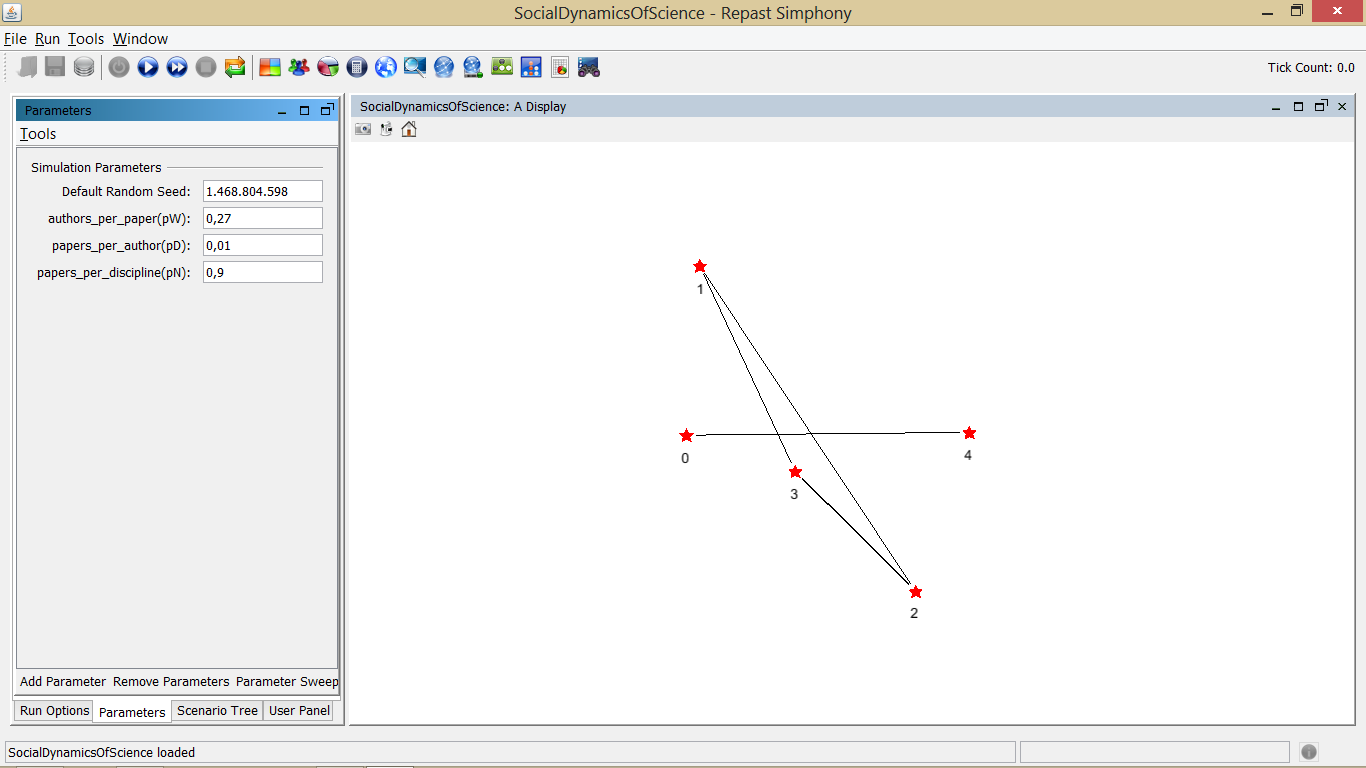
\includegraphics[height= 11cm, width=17cm]{project/images/parameters.png}
\end{figure}
\small{Initial Screenshot and Parameters}
\begin{table}
\begin{tabular}{cc}
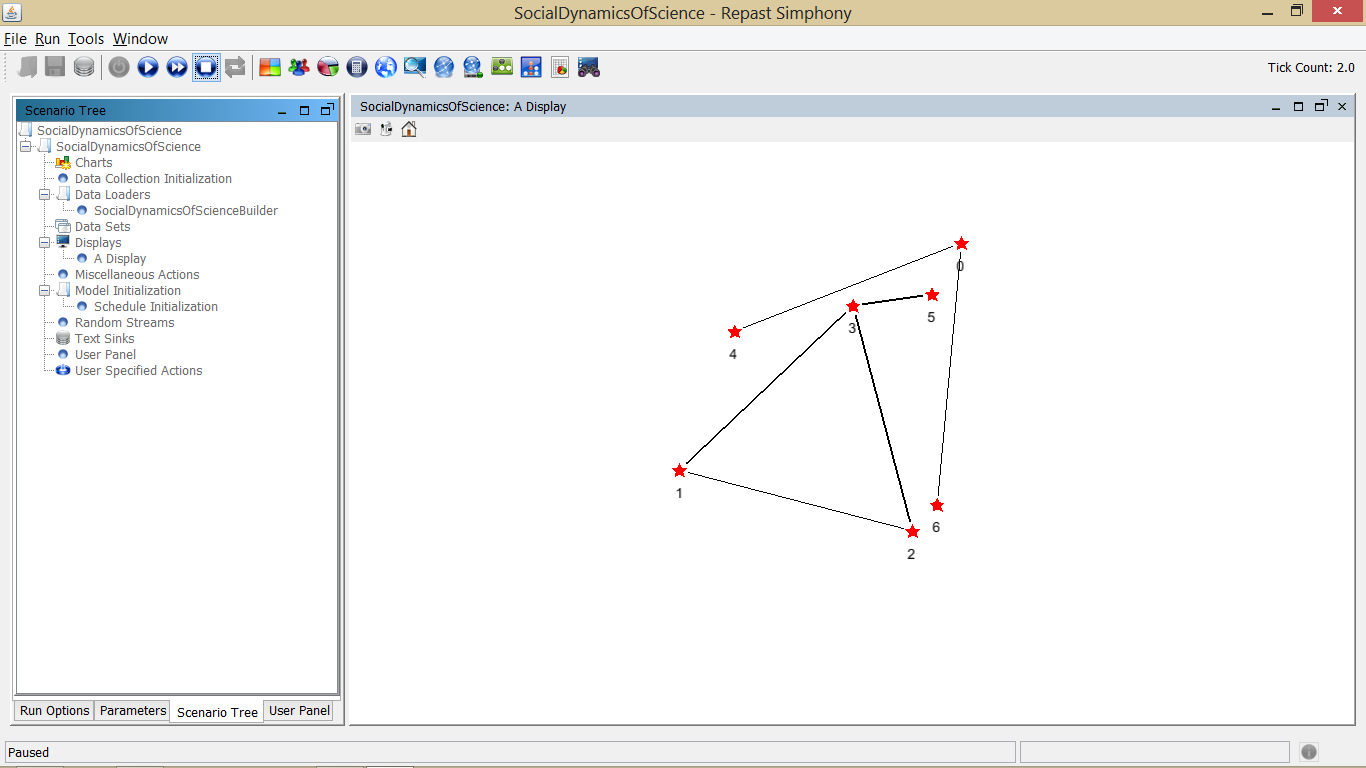
\includegraphics[height= 5cm, width=8cm]{project/images/1.png}
&
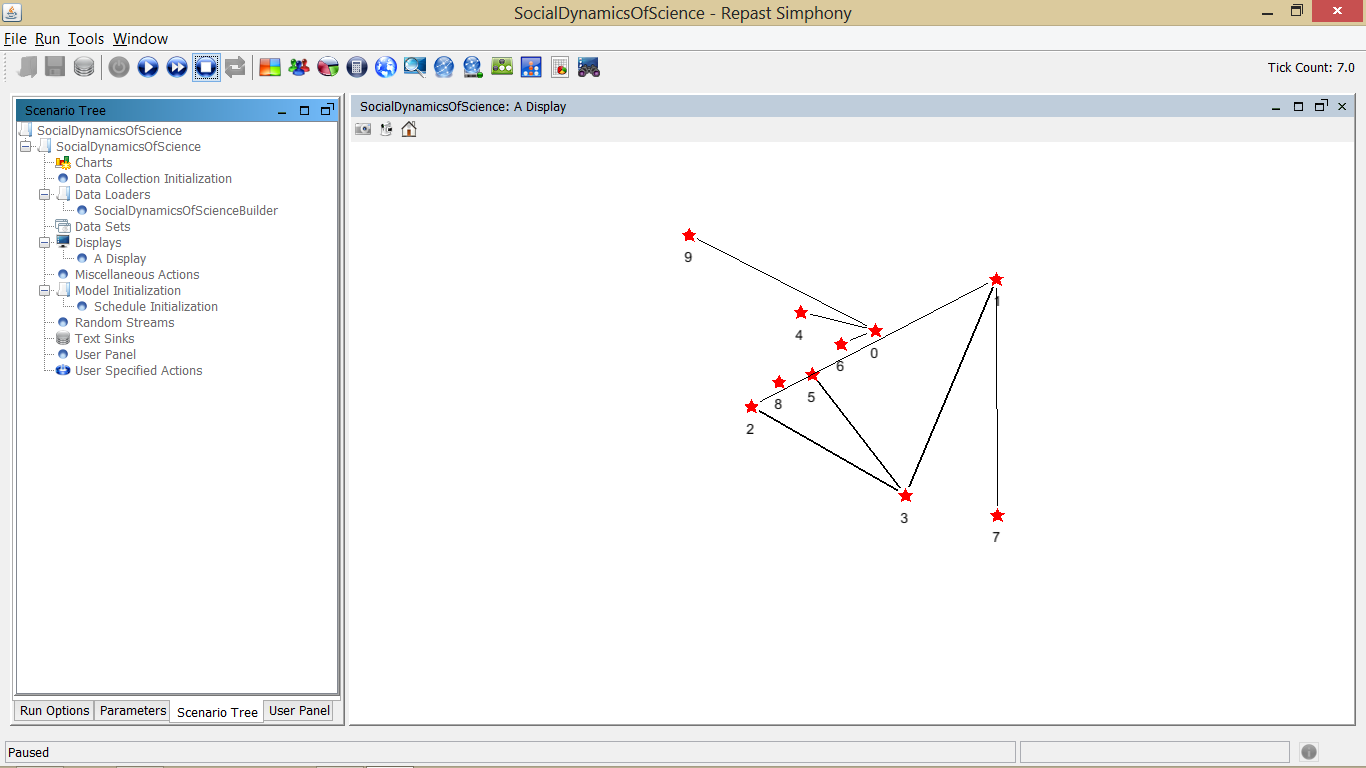
\includegraphics[height= 5cm, width=8cm]{project/images/2.png}
\\ 
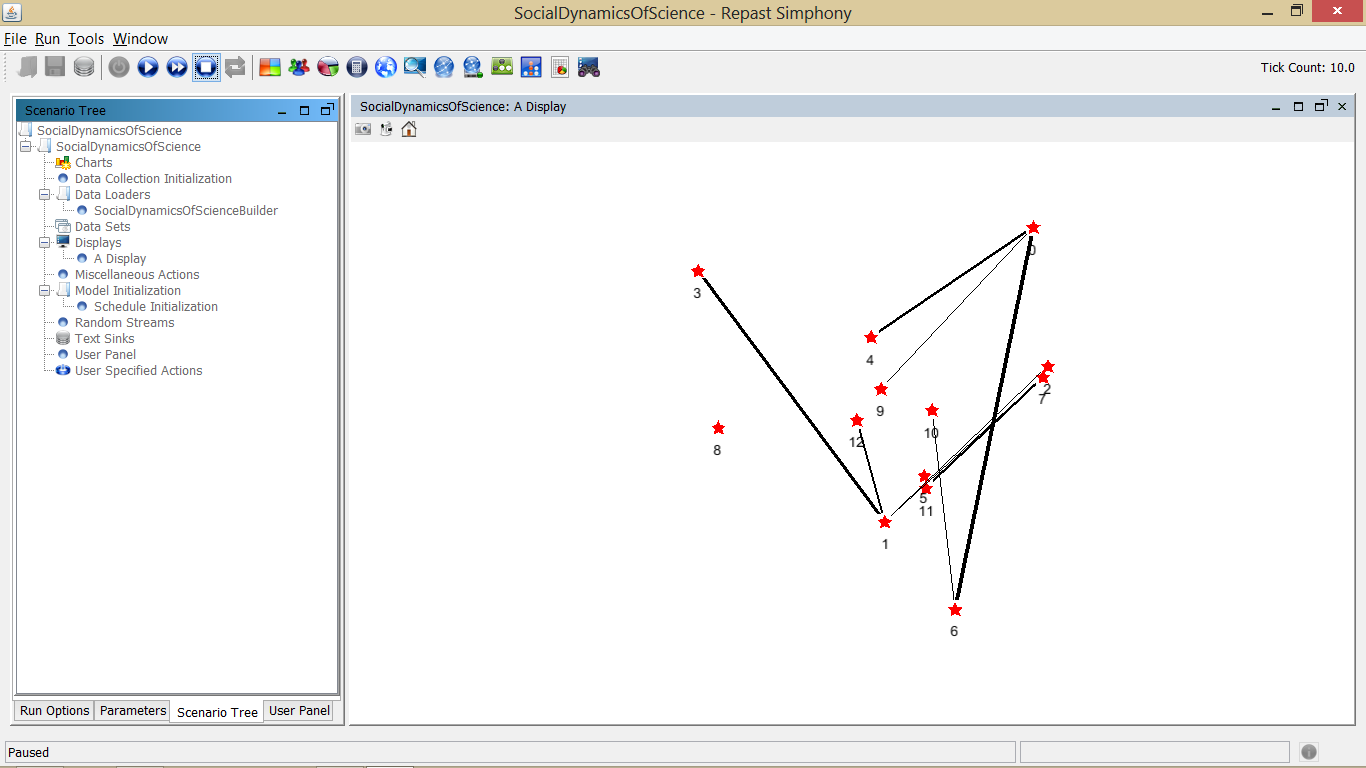
\includegraphics[height= 5cm, width=8cm]{project/images/3.png}
&
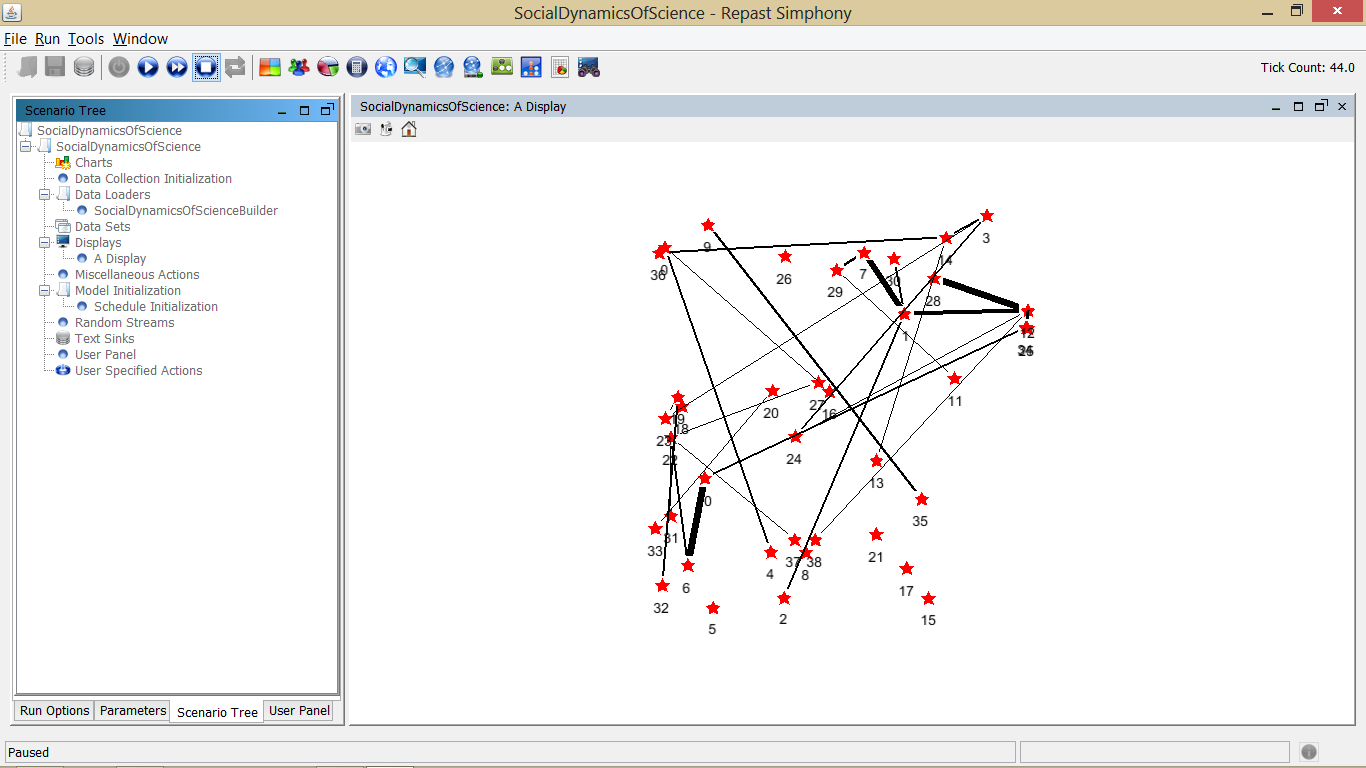
\includegraphics[height= 5cm, width=8cm]{project/images/4.png}
\\ 
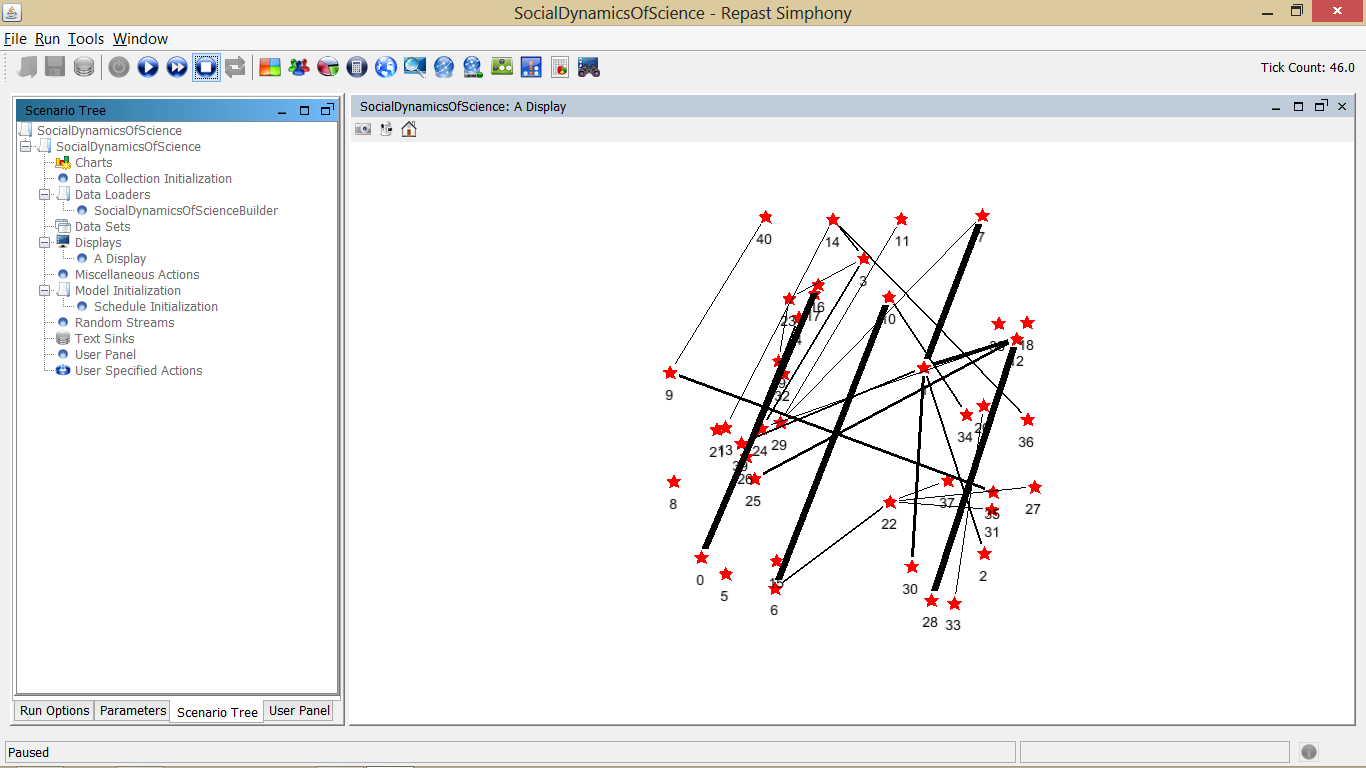
\includegraphics[height= 5cm, width=8cm]{project/images/5.png}
&
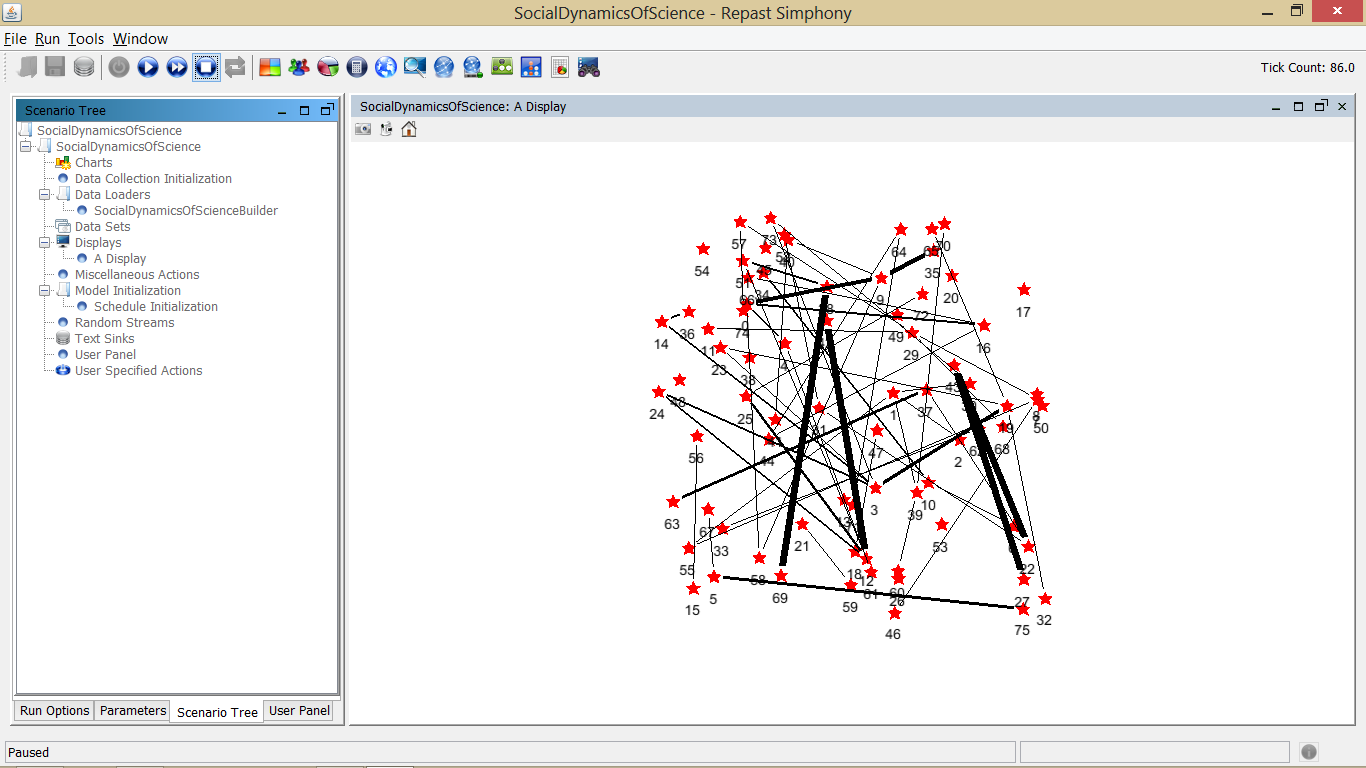
\includegraphics[height= 5cm, width=8cm]{project/images/6.png}

\end{tabular}
\end{table}

\chapter{Future Scope}
\paragraph{}
In future development we can complete the modelize the evalution of diciplines by splitting and merging communities in this network.
These events can be implement with these ideas,
\begin{itemize}
 \item For a split event we select a random discipline with its coauthor network and decide whether a new discipline should emerge from a subset of this community.
We partition the coauthor network into two clusters.
If the modularity of the partition is higher than that of the single discipline, there are more collaborations within each cluster than across the two.
We then split the smaller community as a new discipline.
In this case the papers whose authors are all in the new community are relabeled to reflect the emergent discipline.
Borderline papers with authors in both old and new disciplines are labeled according to the discipline of the majority of authors.
Some authors may as a result belong to both old and new discipline.
 \item For a merge event we randomly select two disciplines with at least one common author.
If the modularity obtained by merging the two groups is higher than that of the partitioned groups, the collaborations across the two communities are stronger than those within each one. The two are then merged into a single new discipline.
In this case all the papers in the two old disciplines are relabeled to reflect the new one.
\end{itemize}
\paragraph{}
In this simulation, when it decides to continue to bias random walk, we just calculate the probability of co-authors with authors who have collaborated before are likely to do so again.
We can develop this probabilistic selection on the bias random walk also with considering these facts,
\begin{itemize}
 \item Authors who have collaborated before are likely to do so again
 \item Authors with common collaborators are likely to collaborate with each other
 \item It is easier to choose collaborators with similar than dissimilar background
 \item Authors with many collaborations have higher probability to gain additional ones
\end{itemize} % adds the Scheduling and Planning page
\addcontentsline{toc}{chapter}{References}
\begin{thebibliography}{99}
\bibitem{} \emph{Social Dynamics of Science}; Xiaoling Sun, Jasleen Kaur, Sta\v{s}a Milojevi\'{c}, Alessandro Flammini, Filippo Menczer
\end{thebibliography} % adds the References page

\end{document}